\section{Pilot Automaton}

\subsection{Parts of a Pilot Automaton}
\begin{figure}[H]
    \centering
    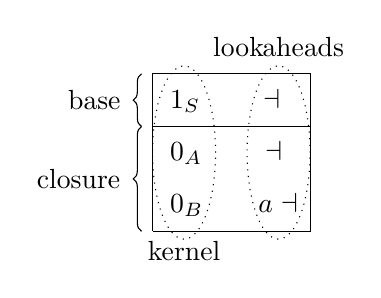
\begin{tikzpicture}
        \draw (0,0) -- (2,0) -- (2,2) -- (0,2) -- (0,0);
        \draw (0,1.33) -- (2,1.33);
        \draw (0.1,1.66) node[anchor=west] {$1_S\qquad \dashv$};
        \draw (0.1,1) node[anchor=west] {$0_A\qquad \dashv$};
        \draw (0.1,0.33) node[anchor=west] {$0_B\qquad a\dashv$};

        \draw[dotted] (0.4,1) ellipse (0.4 and 1.1);
        \draw (0.4,0) node[anchor=north] {kernel};
        \draw[dotted] (1.6,1) ellipse (0.4 and 1.1);
        \draw (1.6,2.1) node[anchor=south] {lookaheads};

        \draw [decorate,decoration={brace,amplitude=3},xshift=-4pt,yshift=0pt]
        (0,1.33) -- (0,2) node [black,midway,xshift=-0.6cm]
        {base};
        \draw [decorate,decoration={brace,amplitude=3},xshift=-4pt,yshift=0pt]
        (0,0) -- (0,1.33) node [black,midway,xshift=-0.8cm]
        {closure};
    \end{tikzpicture}
\end{figure}

\subsection{Closure Function}
Let $C$ be a set of candidates:

\begin{algorithm*}[H]
    \caption{Closure Function}
    \SetAlgoLined
    $K = C$\;
    \Do{nothing changes}{
        \begin{alignat*}{2}
            K = K \cup \{ &\langle 0_B,b \rangle | \exists \langle q,a \rangle \in K \land \\
            & \exists\text{ arc } q\xrightarrow{B} r \text{ in } M \land b \in Ini(L(r).a) \}
        \end{alignat*}
    }
    $closure(C) = K$
\end{algorithm*}

In words:
\begin{itemize}
    \item For each candidate add new candidates with $0_B$ as the kernel.
    \item The lookaheads are $Ini(L(r).a)$, i.e. the characters that can follow $r$, including those due to the nullableness of $r$.
\end{itemize}

\subsection{Construction of the automaton}
Construct the m-states $R = \{I_0, I_1, \ldots\}$ and the state-transition function $\theta$.

\begin{algorithm*}[H]
    \caption{Construction of the automaton}
    \SetAlgoLined
    $R' = \{I_0\}$\;
    \Do{$R \ne R'$}{
        $R = R'$\;
        \For{$I\in R$ and $X\in \Sigma \cup V$}{
            $I' = Closure(\theta(I,X))$\;
            \If{$I' \ne \emptyset$}{
                add arc $I \xrightarrow{X} I'$ to $\theta$\;
                \If{$I'\notin R$}{
                    add $I'$ to $R'$\;
                }
            }
        }
    }
\end{algorithm*}

\newpage

In words:
\begin{itemize}
    \item Start from the initial m-state built from the closure of the initial state of the axiom.
    \item For each m-state add an arc for the exiting transitions to a new m-state considering all the candidates.
    \item Compute and add the closure to the new m-state.
    \item Add the m-state to the automaton \textbf{if not already present}.
\end{itemize}

\textbf{Note}: shift moves do not change the lookaheads, only closures do.
